\documentclass[11pt,a4paper]{article}

\usepackage[utf8]{inputenc}
\usepackage[T1]{fontenc}
\usepackage[spanish,es-tabla,es-noshorthands]{babel}
\usepackage{lmodern}
\usepackage[margin=2.2cm]{geometry}
\usepackage{graphicx}
\usepackage{booktabs}
\usepackage{longtable}
\usepackage{array}
\usepackage{enumitem}
\usepackage[table]{xcolor}
\usepackage{caption}
\usepackage[hidelinks]{hyperref}

\definecolor{verde}{HTML}{1D5C3A}
\definecolor{verdeclaro}{HTML}{E8F4EC}
\newcolumntype{L}[1]{>{\raggedright\arraybackslash}p{#1}}
\newcolumntype{C}[1]{>{\centering\arraybackslash}p{#1}}
\setlist{nosep,leftmargin=*}
\renewcommand{\arraystretch}{1.3}
\setlength{\parskip}{0.5em}
\setlength{\parindent}{0pt}

\newcommand{\hu}[3]{\textbf{Como} #1 \textbf{quiero} #2 \textbf{para} #3}
\newcommand{\dce}[3]{\textbf{Dado} #1, \textbf{cuando} #2, \textbf{entonces} #3}
\newcommand{\criterios}[1]{\subsubsection*{#1}}

\title{\textbf{Laboratorio 3: Elicitación de requerimientos e historias de usuario}\\[0.4em]
\large EcoRuta Cusco: sistema de gestión de recolección de residuos sólidos}
\author{Gisel Dayana Farfan Gomez\\ Ingeniería de Software I}
\date{}

\begin{document}
\maketitle

% ---------------------------------------------------------------
\section{Punto de partida}

Los requerimientos se obtuvieron a partir de los artefactos del Laboratorio 2 (Agile Inception):

\begin{itemize}
  \item \textbf{Roles de usuario:} salen de la lista de stakeholders.
  \item \textbf{Funcionalidades:} salen del alcance del MVP y de la solución del Lean Canvas.
  \item \textbf{Restricciones y criterios de aceptación:} salen de las mitigaciones de los riesgos iniciales (R1 a R9).
\end{itemize}

\begin{center}
\begin{tabular}{L{4.6cm} L{11cm}}
\toprule
\textbf{Rol} & \textbf{Descripción} \\
\midrule
Ciudadano & Vecino del distrito que consulta horarios, recibe alertas y reporta incidencias \\
Operador de camión & Chofer o ayudante que sigue la ruta asignada desde la app móvil \\
Supervisor de limpieza pública & Asigna rutas, monitorea la flota y atiende los reportes ciudadanos \\
Administrador municipal & Configura zonas, rutas, horarios y cuentas del personal \\
Gerente de limpieza pública & Revisa indicadores para tomar decisiones \\
Reciclador formalizado & Consulta puntos y horarios de residuos reciclables \\
\bottomrule
\end{tabular}
\end{center}

% ---------------------------------------------------------------
\section{Identificación de funcionalidades}

Las funcionalidades se agruparon en \textbf{6 épicas}:

{\small
\begin{longtable}{L{2.8cm} L{5.2cm} L{4cm} L{2.4cm}}
\toprule
\textbf{Épica} & \textbf{Funcionalidades} & \textbf{Origen (Lab 2)} & \textbf{Historias} \\
\midrule
\endhead
\textbf{E1. Usuarios y acceso} & Registro de ciudadanos; gestión de cuentas y roles del personal & Stakeholders, riesgo R8 & HU-01, HU-02 \\
\textbf{E2. Planificación del servicio} & Registro de zonas y rutas en mapa; horarios de recojo; asignación de rutas a camiones y operadores & MVP: ``Registro de rutas, zonas y horarios'' & HU-03, HU-04, HU-06 \\
\textbf{E3. Operación en ruta} & Ruta del día en la app del operador; envío de ubicación GPS; registro de paradas atendidas & MVP: ``Seguimiento GPS desde la app del operador'' & HU-07, HU-08, HU-13 \\
\textbf{E4. Información al ciudadano} & Consulta de horarios; alertas de recolección; camión en el mapa; avisos de cambios; puntos de reciclaje; alertas por SMS & MVP: ``Consulta de horarios'' y ``Notificaciones'' & HU-05, HU-10, HU-14, HU-17, HU-18, HU-19 \\
\textbf{E5. Reporte de incidencias} & Reporte de basura acumulada con foto y ubicación; gestión de reportes; seguimiento del reporte & MVP: ``Reporte ciudadano de basura acumulada'' & HU-11, HU-12, HU-15 \\
\textbf{E6. Monitoreo e indicadores} & Panel de flota en tiempo real; indicadores del servicio & MVP: ``Panel de monitoreo y reportes básicos'' & HU-09, HU-16 \\
\bottomrule
\end{longtable}
}

% ---------------------------------------------------------------
\section{Historias de usuario}

Formato: \textbf{Como} [usuario] \textbf{quiero} [funcionalidad] \textbf{para} [beneficio].

{\small
\begin{longtable}{C{1.3cm} L{14.3cm}}
\toprule
\textbf{ID} & \textbf{Historia de usuario} \\
\midrule
\endhead
HU-01 & \hu{ciudadano}{registrarme con mi correo o celular y mi dirección}{recibir la información de recojo de mi zona.} \\
HU-02 & \hu{administrador municipal}{crear cuentas para operadores y supervisores y asignarles un rol}{que cada uno acceda solo a las funciones que le corresponden.} \\
HU-03 & \hu{administrador municipal}{registrar zonas y rutas de recolección sobre un mapa}{planificar el recorrido de los camiones.} \\
HU-04 & \hu{administrador municipal}{definir los días y horarios de recojo de cada zona por tipo de residuo}{que el servicio sea predecible.} \\
HU-05 & \hu{ciudadano}{consultar el horario de recojo escribiendo mi dirección}{sacar mi basura a tiempo.} \\
HU-06 & \hu{supervisor}{asignar cada ruta a un camión y a un operador por día}{organizar el servicio.} \\
HU-07 & \hu{operador de camión}{ver en mi celular la ruta del día con las paradas en orden}{seguir el recorrido sin perderme.} \\
HU-08 & \hu{operador de camión}{que la app envíe mi ubicación automáticamente mientras hago la ruta}{que la municipalidad y los vecinos sepan dónde está el camión.} \\
HU-09 & \hu{supervisor}{ver en un mapa la ubicación en tiempo real de todos los camiones}{saber si están cumpliendo sus rutas.} \\
HU-10 & \hu{ciudadano}{recibir una alerta cuando el camión esté cerca de mi casa}{sacar mi basura a tiempo.} \\
HU-11 & \hu{ciudadano}{reportar un punto de basura acumulada con una foto y su ubicación}{que la municipalidad lo atienda.} \\
HU-12 & \hu{supervisor}{ver los reportes ciudadanos en una lista y en un mapa y cambiar su estado}{organizar su atención.} \\
HU-13 & \hu{operador de camión}{marcar cada parada como atendida o no atendida}{dejar registro del servicio realizado.} \\
HU-14 & \hu{ciudadano}{ver en el mapa dónde está el camión de mi zona}{saber cuánto falta para que pase.} \\
HU-15 & \hu{ciudadano}{ver el estado de mis reportes}{saber si fueron atendidos.} \\
HU-16 & \hu{gerente de limpieza pública}{ver indicadores del servicio por zona y por fecha}{tomar decisiones sobre rutas y recursos.} \\
HU-17 & \hu{administrador municipal}{publicar avisos de cambios temporales de horario}{que los vecinos se enteren a tiempo.} \\
HU-18 & \hu{reciclador formalizado}{consultar los puntos y horarios de recojo de residuos reciclables}{organizar mi recorrido.} \\
HU-19 & \hu{ciudadano sin smartphone}{recibir las alertas por SMS o WhatsApp}{no quedar fuera del servicio.} \\
\bottomrule
\end{longtable}
}

\subsection{Verificación de calidad (INVEST)}

Cada historia se revisó con el criterio \textbf{INVEST}:

{\small
\begin{longtable}{L{3.2cm} L{12.4cm}}
\toprule
\textbf{Criterio} & \textbf{Cómo se aplicó} \\
\midrule
\endhead
\textbf{I}ndependiente & Cada historia entrega una funcionalidad completa. Las dependencias se resolvieron con el orden del backlog (por ejemplo, HU-03 va antes que HU-04) \\
\textbf{N}egociable & Las historias dicen \textit{qué} se necesita, no \textit{cómo} implementarlo (no fijan tecnología ni pantallas) \\
\textbf{V}aliosa & Todas tienen un ``para'' con un beneficio concreto para un rol real \\
\textbf{E}stimable & Todas tienen story points asignados \\
\textbf{S}mall (pequeña) & Ninguna supera 8 puntos, así que cada una cabe en un sprint \\
\textbf{T}esteable & Todas tienen criterios de aceptación verificables (sección~\ref{sec:criterios}) \\
\bottomrule
\end{longtable}
}

% ---------------------------------------------------------------
\section{Priorización: Product Backlog inicial}

\subsection{Criterios usados}

\begin{itemize}
  \item \textbf{MoSCoW:}
  \begin{itemize}
    \item \textbf{Must:} sin esto el MVP no funciona.
    \item \textbf{Should:} importante, pero el MVP funciona sin ello.
    \item \textbf{Could:} deseable si hay tiempo.
    \item \textbf{Won't:} fuera de esta versión.
  \end{itemize}
  \item \textbf{Story points (SP):} escala de Fibonacci (1, 2, 3, 5, 8). Mide el esfuerzo relativo, no horas.
  \item \textbf{Orden dentro de cada prioridad:}
  \begin{enumerate}
    \item Dependencias: primero los datos base (usuarios, zonas, rutas).
    \item Valor para el objetivo principal del Lab 2: ``que la basura se recoja a tiempo''.
    \item Riesgo: lo más incierto técnicamente (GPS) se aborda temprano.
  \end{enumerate}
\end{itemize}

\subsection{Backlog ordenado}

{\small
\begin{longtable}{C{1.1cm} C{1.3cm} L{4.9cm} C{1.1cm} L{2.4cm} C{1.7cm} C{0.7cm}}
\toprule
\textbf{Orden} & \textbf{ID} & \textbf{Historia (resumen)} & \textbf{Épica} & \textbf{Rol} & \textbf{Prioridad} & \textbf{SP} \\
\midrule
\endhead
1 & HU-01 & Registro de ciudadanos & E1 & Ciudadano & Must & 3 \\
2 & HU-02 & Cuentas y roles del personal & E1 & Administrador & Must & 3 \\
3 & HU-03 & Zonas y rutas en mapa & E2 & Administrador & Must & 8 \\
4 & HU-04 & Horarios de recojo por zona & E2 & Administrador & Must & 5 \\
5 & HU-05 & Consulta de horario por dirección & E4 & Ciudadano & Must & 3 \\
6 & HU-06 & Asignación de rutas a camión y operador & E2 & Supervisor & Must & 3 \\
7 & HU-07 & Ruta del día en la app del operador & E3 & Operador & Must & 5 \\
8 & HU-08 & Envío automático de ubicación GPS & E3 & Operador & Must & 8 \\
9 & HU-09 & Monitoreo de la flota en tiempo real & E6 & Supervisor & Must & 8 \\
10 & HU-10 & Alerta de camión cercano & E4 & Ciudadano & Must & 8 \\
11 & HU-11 & Reporte de basura acumulada & E5 & Ciudadano & Must & 5 \\
12 & HU-12 & Gestión de reportes ciudadanos & E5 & Supervisor & Must & 5 \\
\midrule
13 & HU-13 & Registro de paradas atendidas & E3 & Operador & Should & 3 \\
14 & HU-14 & Camión en el mapa para el ciudadano & E4 & Ciudadano & Should & 5 \\
15 & HU-15 & Seguimiento del reporte & E5 & Ciudadano & Should & 3 \\
16 & HU-16 & Indicadores del servicio & E6 & Gerente & Should & 5 \\
\midrule
17 & HU-17 & Avisos de cambios de horario & E4 & Administrador & Could & 3 \\
18 & HU-18 & Puntos de reciclaje & E4 & Reciclador & Could & 2 \\
\midrule
19 & HU-19 & Alertas por SMS o WhatsApp & E4 & Ciudadano & Won't & 5 \\
\bottomrule
\end{longtable}
}

\subsection{Resumen}

\begin{center}
\begin{tabular}{L{4.5cm} C{2.5cm} C{2.8cm}}
\toprule
\textbf{Prioridad} & \textbf{Historias} & \textbf{Story points} \\
\midrule
Must & 12 & 64 \\
Should & 4 & 16 \\
Could & 2 & 5 \\
Won't (esta versión) & 1 & 5 \\
\midrule
\textbf{Total} & \textbf{19} & \textbf{90} \\
\bottomrule
\end{tabular}
\end{center}

\begin{itemize}
  \item \textbf{Primera versión (MVP):} las 12 historias \textit{Must} (HU-01 a HU-12). Con ellas se cumple el ciclo completo: la municipalidad planifica, el camión transmite su ubicación, el ciudadano recibe la alerta y puede reportar incidencias.
  \item \textbf{HU-19 queda como \textit{Won't}:} el envío de SMS tiene un costo por mensaje que hoy no está presupuestado. Se mantiene en el backlog porque es la mitigación del riesgo R1 (baja adopción) y se retomará si la adopción por la app es baja.
\end{itemize}

% ---------------------------------------------------------------
\clearpage
\section{Trabajo extra: criterios de aceptación}\label{sec:criterios}

Formato: \textbf{Dado} [contexto] \textbf{cuando} [acción] \textbf{entonces} [resultado esperado].

\criterios{HU-01: Registro de ciudadanos}
\begin{enumerate}
  \item \dce{que ingreso nombre, correo o celular, contraseña y dirección válidos}{confirmo el registro}{se crea mi cuenta y el sistema me asigna la zona de mi dirección.}
  \item \dce{que el correo o celular ya está registrado}{intento registrarme}{el sistema me lo indica y me ofrece iniciar sesión.}
  \item \dce{que mi dirección no tiene numeración}{la registro}{puedo marcar mi vivienda directamente en el mapa.}
  \item \dce{que no acepto la política de privacidad}{intento registrarme}{no se crea la cuenta. Solo se piden los datos mínimos (Ley 29733, riesgo R8).}
\end{enumerate}

\criterios{HU-02: Cuentas y roles del personal}
\begin{enumerate}
  \item \dce{que creo una cuenta con rol ``operador''}{esa persona inicia sesión}{solo ve la app de ruta, no el panel municipal.}
  \item \dce{que desactivo una cuenta}{el usuario intenta iniciar sesión}{el acceso es denegado.}
  \item \dce{que soy ciudadano}{intento entrar al panel municipal}{el sistema me lo impide.}
\end{enumerate}

\criterios{HU-03: Zonas y rutas en mapa}
\begin{enumerate}
  \item \dce{que dibujo el área de una zona en el mapa}{la guardo con un nombre}{queda disponible para asignarle horarios y rutas.}
  \item \dce{que creo una ruta}{agrego sus paradas en orden}{el mapa muestra el recorrido y su distancia aproximada.}
  \item \dce{que una nueva zona se superpone con otra existente}{intento guardarla}{el sistema me advierte (riesgo R6).}
\end{enumerate}

\criterios{HU-04: Horarios de recojo por zona}
\begin{enumerate}
  \item \dce{que selecciono una zona}{registro días, rango horario y tipo de residuo (general o reciclable)}{el horario queda visible para los ciudadanos de esa zona.}
  \item \dce{que la hora de fin es anterior a la de inicio}{intento guardar}{el sistema no lo permite.}
  \item \dce{que modifico un horario}{guardo el cambio}{la consulta de horarios muestra el nuevo valor de inmediato.}
\end{enumerate}

\criterios{HU-05: Consulta de horario por dirección}
\begin{enumerate}
  \item \dce{que mi dirección está dentro de una zona registrada}{la busco}{veo los días, el rango horario y el tipo de residuo.}
  \item \dce{que mi dirección está fuera de las zonas registradas}{la busco}{el sistema muestra ``zona sin horario registrado''.}
  \item \dce{que no tengo cuenta}{entro a la web}{igual puedo consultar el horario (sin iniciar sesión).}
\end{enumerate}

\criterios{HU-06: Asignación de rutas a camión y operador}
\begin{enumerate}
  \item \dce{que la ruta, el camión y el operador están disponibles}{hago la asignación para una fecha}{la ruta aparece en la app del operador ese día.}
  \item \dce{que el camión ya tiene otra ruta en el mismo horario}{intento asignarlo}{el sistema impide la asignación.}
  \item \dce{que reasigno una ruta a otro operador}{guardo el cambio}{el operador anterior deja de verla y el nuevo la recibe.}
\end{enumerate}

\criterios{HU-07: Ruta del día en la app del operador}
\begin{enumerate}
  \item \dce{que tengo una ruta asignada}{abro la app}{veo el mapa del recorrido y la lista de paradas en orden, en no más de dos toques (riesgo R3).}
  \item \dce{que no tengo conexión}{abro la app}{veo la ruta que se descargó previamente (riesgo R4).}
  \item \dce{que no tengo ruta asignada}{abro la app}{veo el mensaje ``No tienes rutas asignadas para hoy''.}
\end{enumerate}

\criterios{HU-08: Envío automático de ubicación GPS}
\begin{enumerate}
  \item \dce{que inicié la ruta}{el camión está en movimiento}{la app envía la ubicación cada 30 segundos sin que yo haga nada.}
  \item \dce{que pierdo la señal}{recupero la conexión}{las ubicaciones guardadas se sincronizan en orden (riesgos R2 y R4).}
  \item \dce{que finalizo la ruta}{confirmo el fin}{la app deja de enviar la ubicación.}
\end{enumerate}

\criterios{HU-09: Monitoreo de la flota en tiempo real}
\begin{enumerate}
  \item \dce{que hay camiones en ruta}{abro el panel}{veo cada camión en el mapa con su ruta, su operador y su porcentaje de avance.}
  \item \dce{que un camión no envía ubicación por más de 5 minutos}{reviso el panel}{aparece como ``sin señal'' con su última ubicación conocida y la hora (riesgo R2).}
  \item \dce{que el panel está abierto}{llegan nuevas ubicaciones}{el mapa se actualiza al menos una vez por minuto sin recargar la página.}
\end{enumerate}

\criterios{HU-10: Alerta de camión cercano}
\begin{enumerate}
  \item \dce{que tengo las alertas activadas}{el camión de mi zona está a 10 minutos de mi dirección}{recibo una notificación en el celular.}
  \item \dce{que quiero más o menos anticipación}{entro a configuración}{puedo elegir 5, 10 o 15 minutos, o desactivar las alertas.}
  \item \dce{que el camión pasa varias veces cerca de mi casa en el mismo recorrido}{se generan las alertas}{recibo una sola notificación.}
\end{enumerate}

\criterios{HU-11: Reporte de basura acumulada}
\begin{enumerate}
  \item \dce{que adjunto una foto y la ubicación (GPS o marcada en el mapa)}{envío el reporte}{queda registrado como ``Pendiente'' y recibo un número de seguimiento.}
  \item \dce{que no adjunto foto o ubicación}{intento enviar}{el sistema no lo permite (riesgo R7).}
  \item \dce{que ya envié 5 reportes en el día}{intento enviar otro}{el sistema me indica que alcancé el límite diario (riesgo R7).}
\end{enumerate}

\criterios{HU-12: Gestión de reportes ciudadanos}
\begin{enumerate}
  \item \dce{que hay reportes nuevos}{abro la bandeja}{veo la foto, la ubicación, la fecha y el estado de cada uno, ordenados del más antiguo al más reciente.}
  \item \dce{que cambio el estado de un reporte (Pendiente $\rightarrow$ En atención $\rightarrow$ Atendido)}{guardo}{quedan registrados la fecha y el responsable del cambio.}
  \item \dce{que rechazo un reporte}{guardo}{el sistema me obliga a indicar el motivo.}
\end{enumerate}

\criterios{HU-13: Registro de paradas atendidas}
\begin{enumerate}
  \item \dce{que llego a una parada}{la marco como atendida}{se registran la hora y la ubicación.}
  \item \dce{que no pude atender una parada}{la marco como no atendida}{debo elegir un motivo (calle bloqueada, camión lleno u otro) y el supervisor lo ve en el panel.}
  \item \dce{que no tengo conexión}{marco una parada}{el registro se guarda y se envía al recuperar la señal.}
\end{enumerate}

\criterios{HU-14: Camión en el mapa para el ciudadano}
\begin{enumerate}
  \item \dce{que el camión de mi zona está en ruta}{abro el mapa}{veo su posición y el tiempo estimado de llegada a mi dirección.}
  \item \dce{que no hay un camión en ruta en mi zona}{abro el mapa}{veo la fecha y hora del próximo recojo.}
  \item \dce{que el camión perdió la señal}{abro el mapa}{veo su ``última ubicación conocida'' con la hora.}
\end{enumerate}

\criterios{HU-15: Seguimiento del reporte}
\begin{enumerate}
  \item \dce{que envié reportes}{abro ``Mis reportes''}{veo cada uno con su estado y la fecha del último cambio.}
  \item \dce{que mi reporte pasa a ``Atendido''}{el supervisor guarda el cambio}{recibo una notificación.}
  \item \dce{que mi reporte es rechazado}{recibo la notificación}{veo el motivo del rechazo.}
\end{enumerate}

\criterios{HU-16: Indicadores del servicio}
\begin{enumerate}
  \item \dce{que elijo un rango de fechas}{abro los indicadores}{veo el porcentaje de rutas completadas a tiempo, los reportes recibidos vs.\ atendidos y el tiempo promedio de atención.}
  \item \dce{que selecciono una zona}{aplico el filtro}{los indicadores se recalculan solo para esa zona.}
  \item \dce{que necesito presentar los resultados}{pulso ``Exportar''}{descargo los indicadores en Excel o PDF.}
\end{enumerate}

\criterios{HU-17: Avisos de cambios de horario}
\begin{enumerate}
  \item \dce{que creo un aviso para ciertas zonas y fechas}{lo publico}{los ciudadanos de esas zonas reciben una notificación.}
  \item \dce{que hay un aviso vigente}{un ciudadano consulta su horario}{ve el aviso junto al horario.}
  \item \dce{que pasó la fecha final del aviso}{se consulta el horario}{el aviso ya no se muestra.}
\end{enumerate}

\criterios{HU-18: Puntos de reciclaje}
\begin{enumerate}
  \item \dce{que entro a la sección de reciclaje}{se carga el mapa}{veo los puntos de acopio con sus días y horarios.}
  \item \dce{que selecciono una zona}{aplico el filtro}{solo veo los puntos de esa zona.}
\end{enumerate}

\criterios{HU-19: Alertas por SMS o WhatsApp (Won't en esta versión)}
\begin{enumerate}
  \item \dce{que registré mi celular y elegí SMS como canal}{el camión se acerca}{recibo la alerta por SMS.}
  \item \dce{que no tengo la app instalada}{me registro por la web}{puedo elegir SMS o WhatsApp como canal de alertas.}
\end{enumerate}

% ---------------------------------------------------------------
\section{Product Backlog en Jira}

El Product Backlog se registró en \textbf{Jira}, en el espacio Scrum \textbf{EcoRuta Cusco (ECO)}
(\href{https://ing-software1-residuos.atlassian.net/jira/software/projects/ECO/boards/2/backlog}{\textcolor{verde}{ver backlog en Jira}}).

\begin{itemize}
  \item \textbf{Épicas:} E1 a E6 (ECO-1 a ECO-6).
  \item \textbf{Historias:} HU-01 a HU-19 (ECO-7 a ECO-25), cada una con:
  \begin{itemize}
    \item la historia y sus criterios de aceptación en la descripción;
    \item su épica, sus story points y su prioridad;
    \item etiquetas con la prioridad MoSCoW y el rol de usuario.
  \end{itemize}
  \item \textbf{Prioridad en Jira:} se asignó según MoSCoW: Must $\rightarrow$ Highest, Should $\rightarrow$ High, Could $\rightarrow$ Medium, Won't $\rightarrow$ Lowest.
  \item \textbf{Orden del backlog:} el mismo de la sección 4. Las historias quedan listas para planificar el primer sprint.
\end{itemize}

El backlog también se exportó en \texttt{docs/backlog/product-backlog-jira.csv}, que puede importarse en Jira desde \textit{Importar incidencias desde CSV}.

\begin{figure}[h]
  \centering
  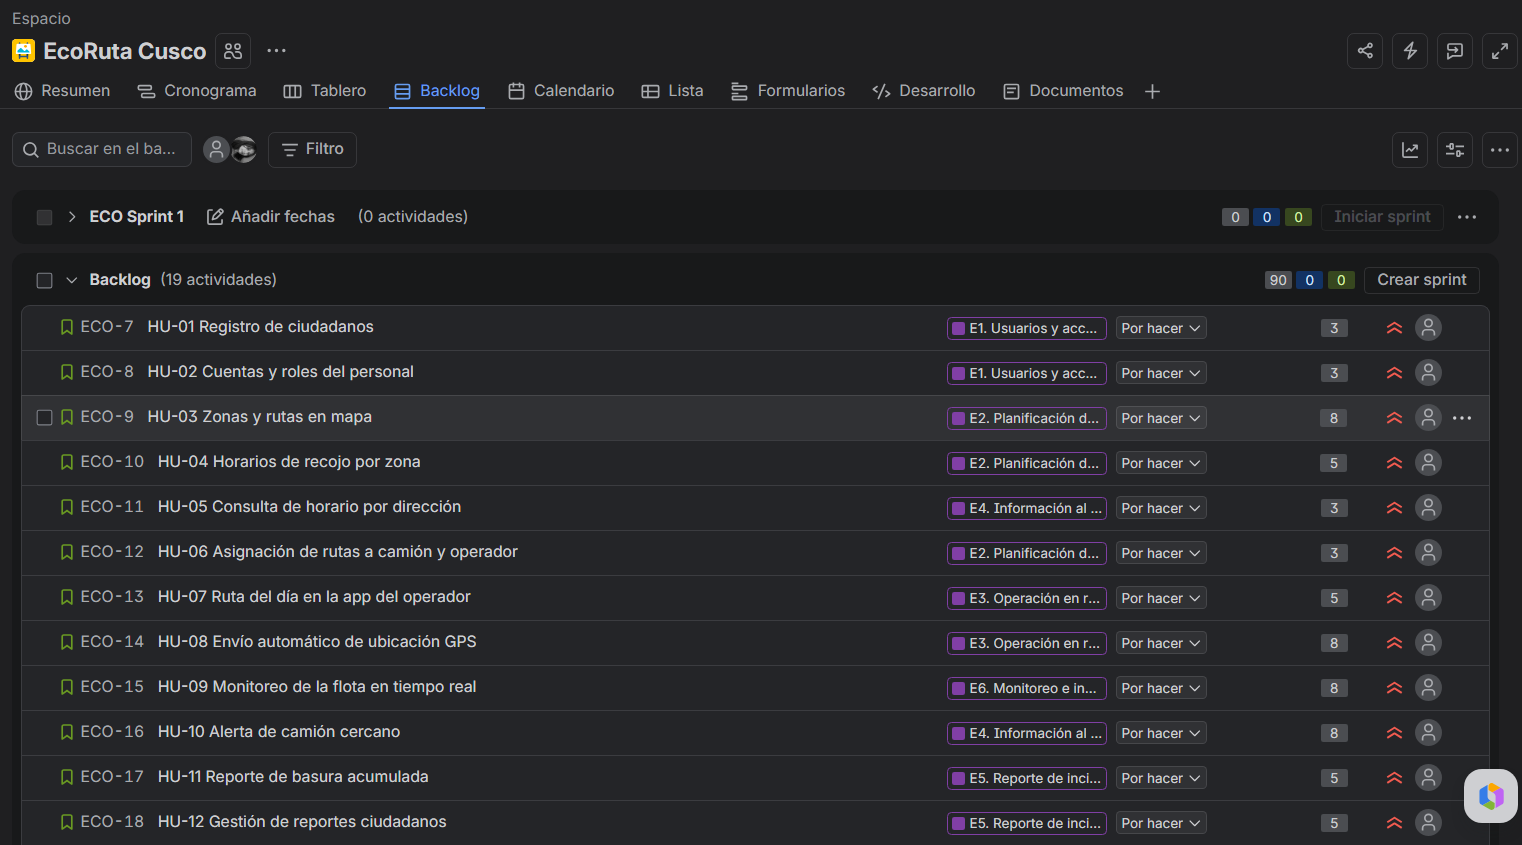
\includegraphics[width=\linewidth]{../img/jira-backlog-1.png}
  \caption{Product Backlog en Jira: historias \textit{Must}.}
\end{figure}

\begin{figure}[h]
  \centering
  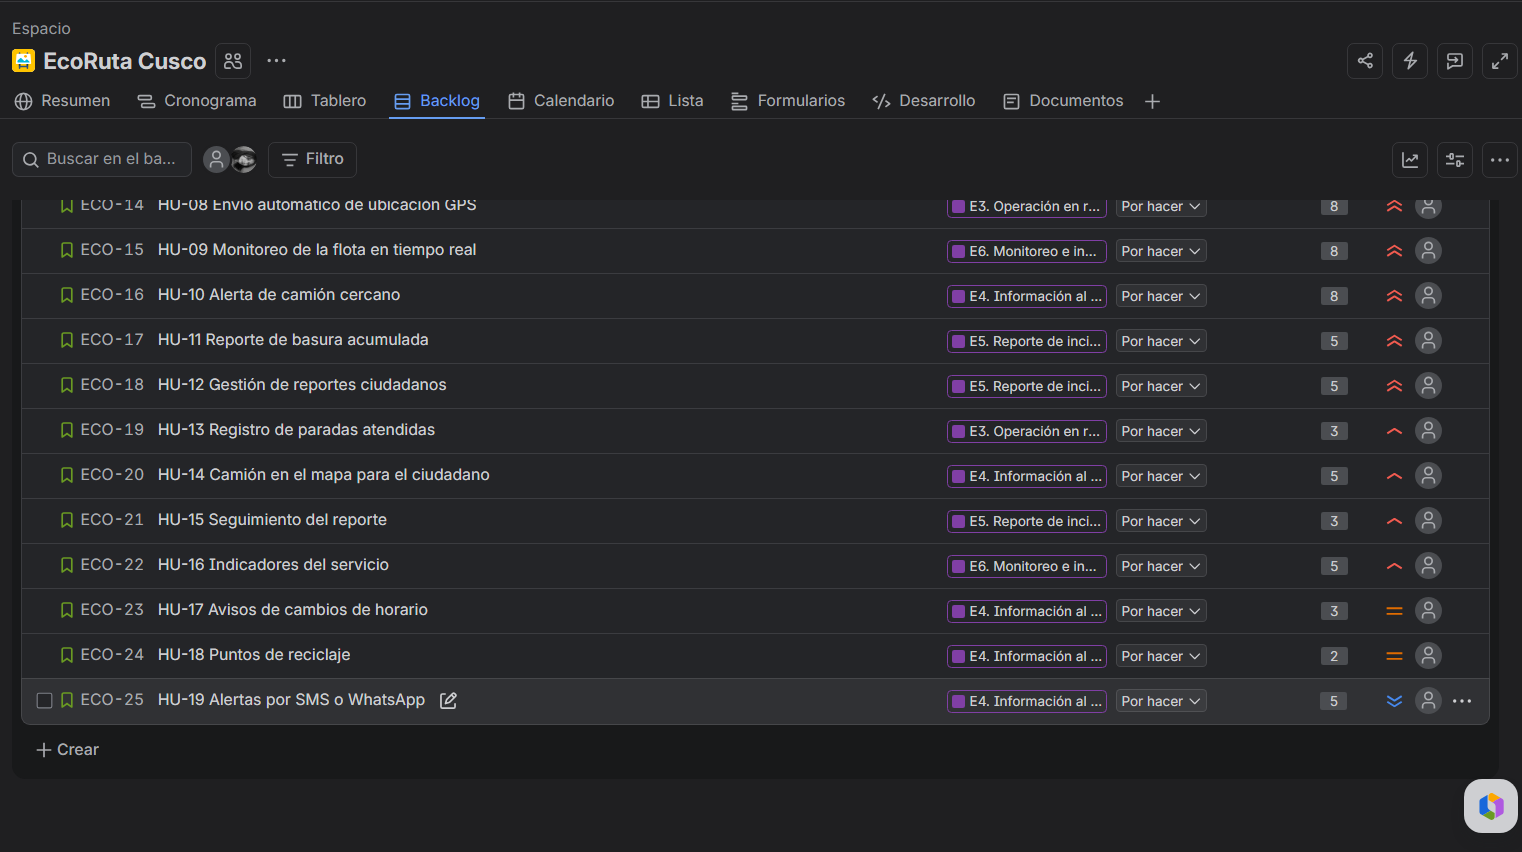
\includegraphics[width=\linewidth]{../img/jira-backlog-2.png}
  \caption{Product Backlog en Jira: historias \textit{Should}, \textit{Could} y \textit{Won't}.}
\end{figure}

\end{document}
